%\documentclass{article}
%\usepackage{graphicx}
%\usepackage{caption,rotating}
%\usepackage{subfigure}
%\begin{document}
\begin{figure}
\begin{turn}{90}
\begin{minipage}[c][\textwidth][c]{\textheight}
 \subfigure[Unaligned staple crimp type]{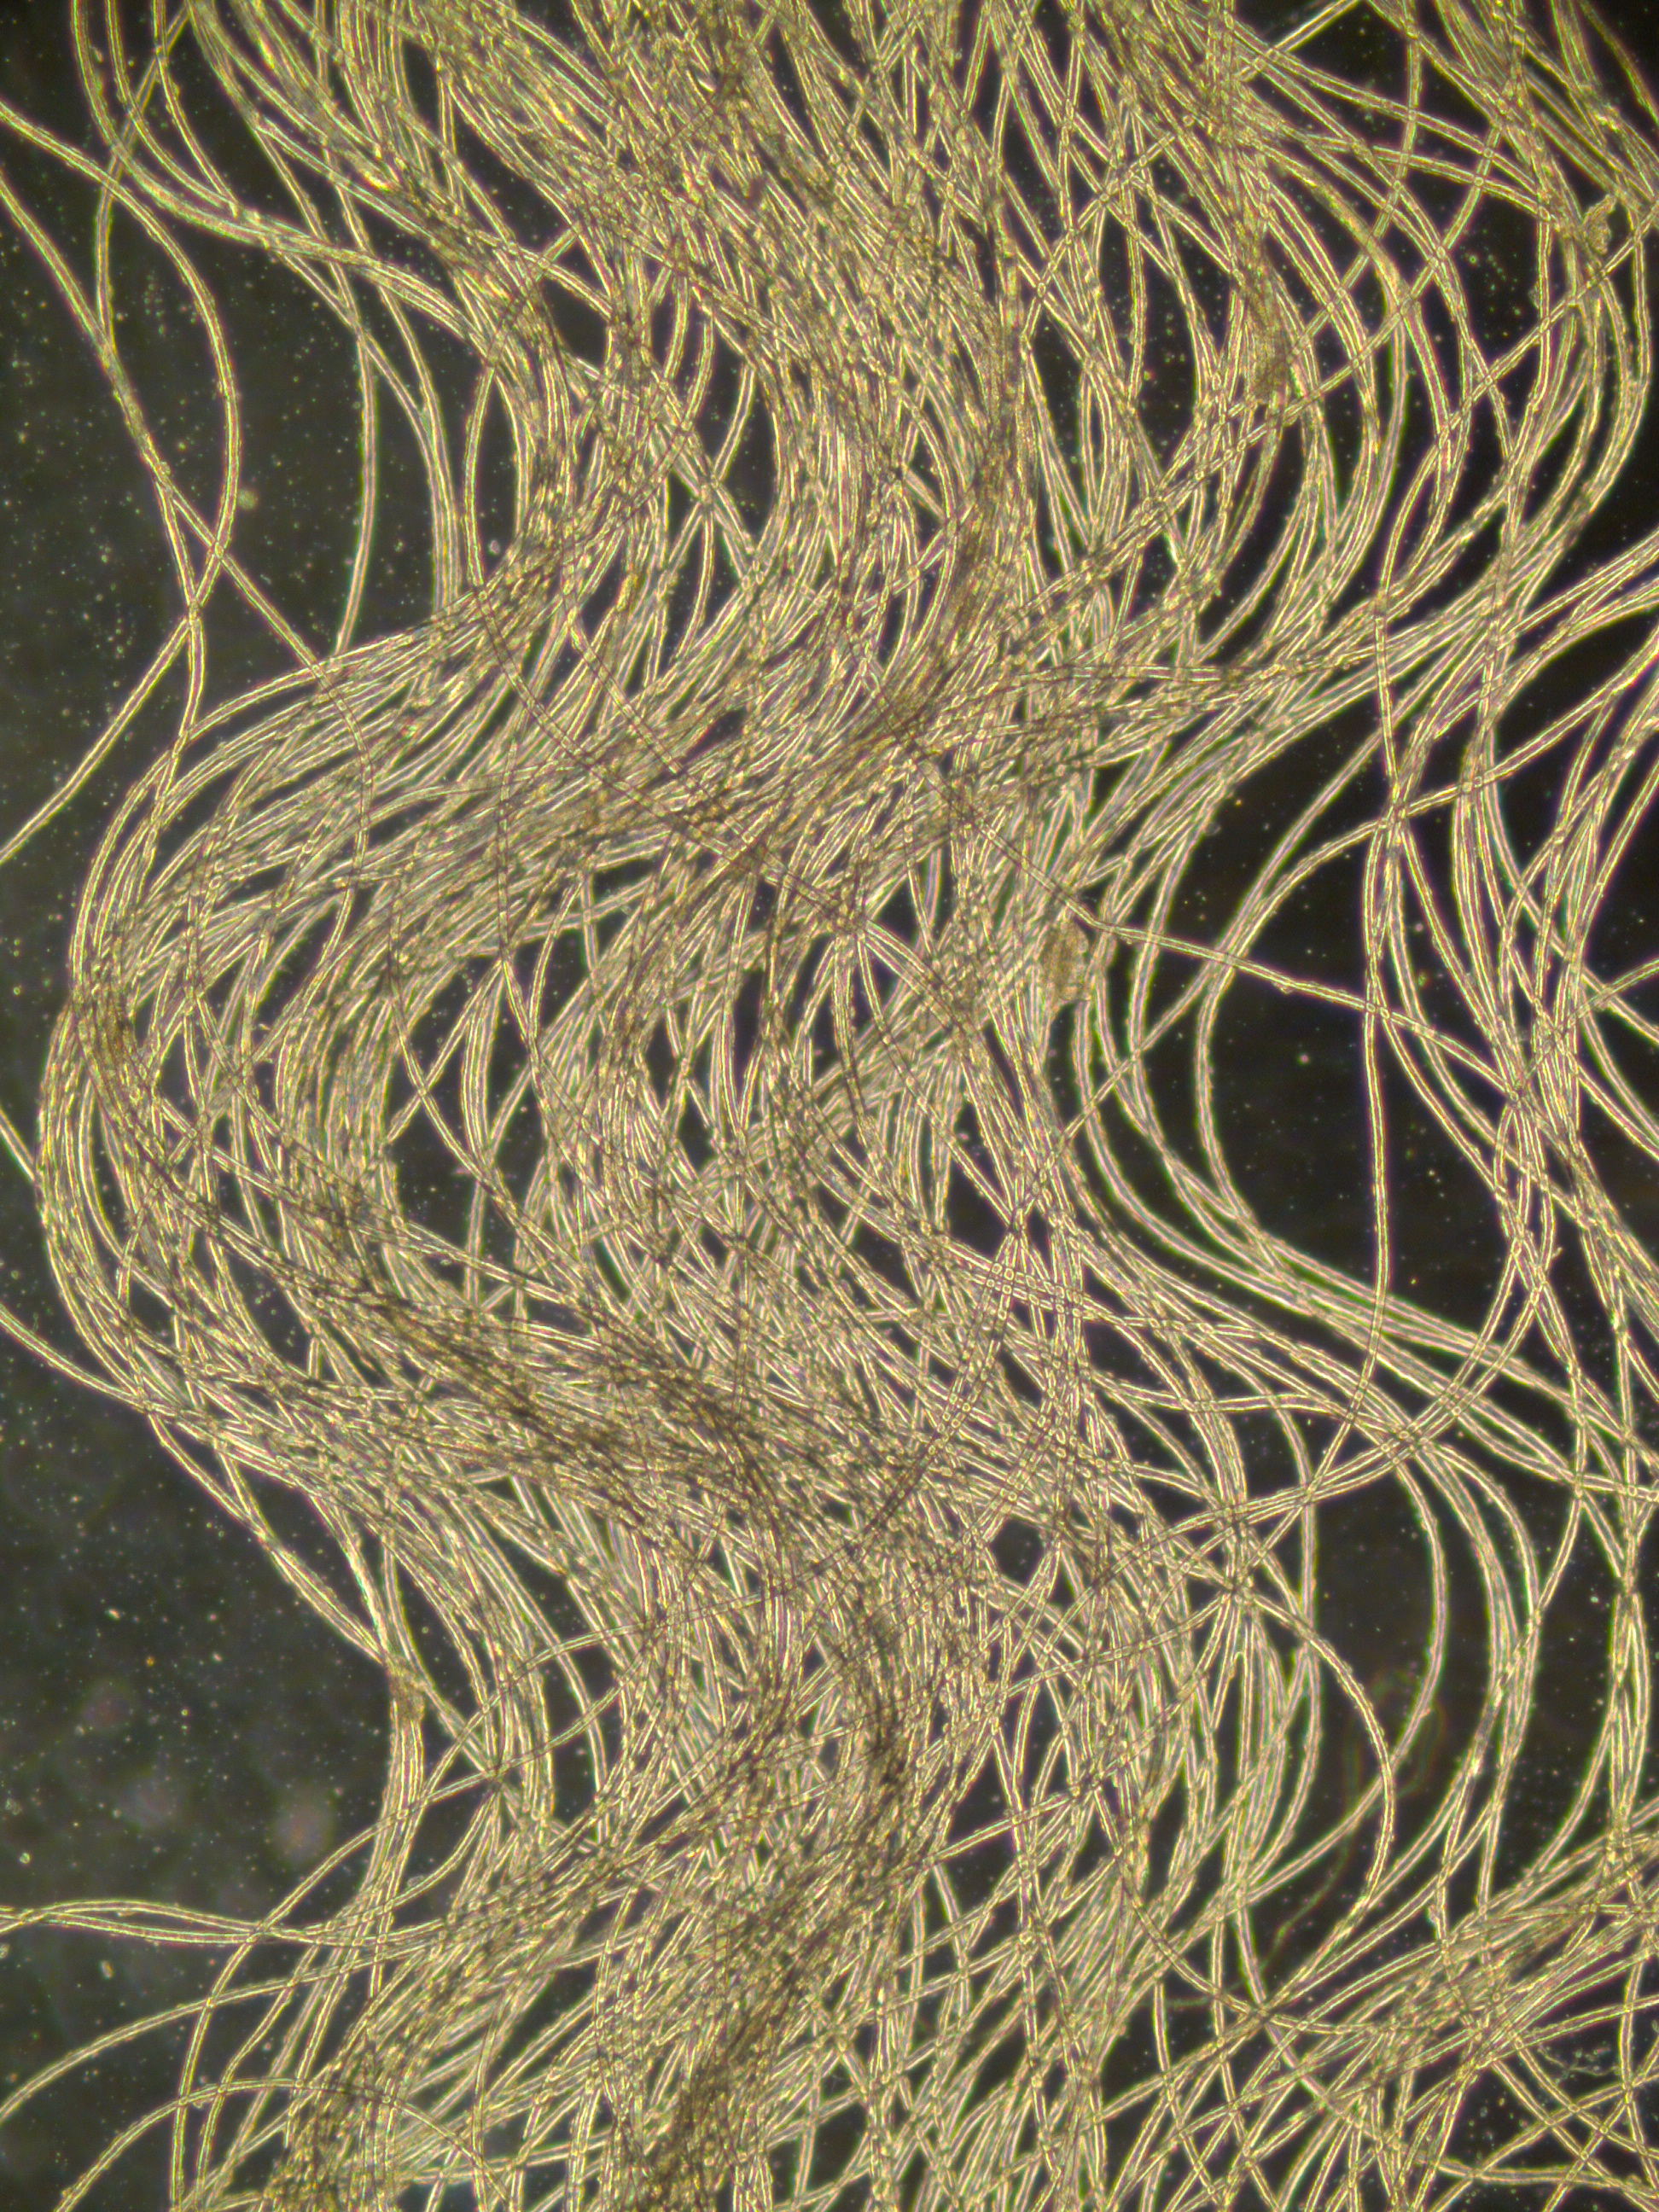
\includegraphics[scale=0.38]{figfibresunalignedrot.jpg}}\hfill
 \subfigure[Stretched staple crimp type]{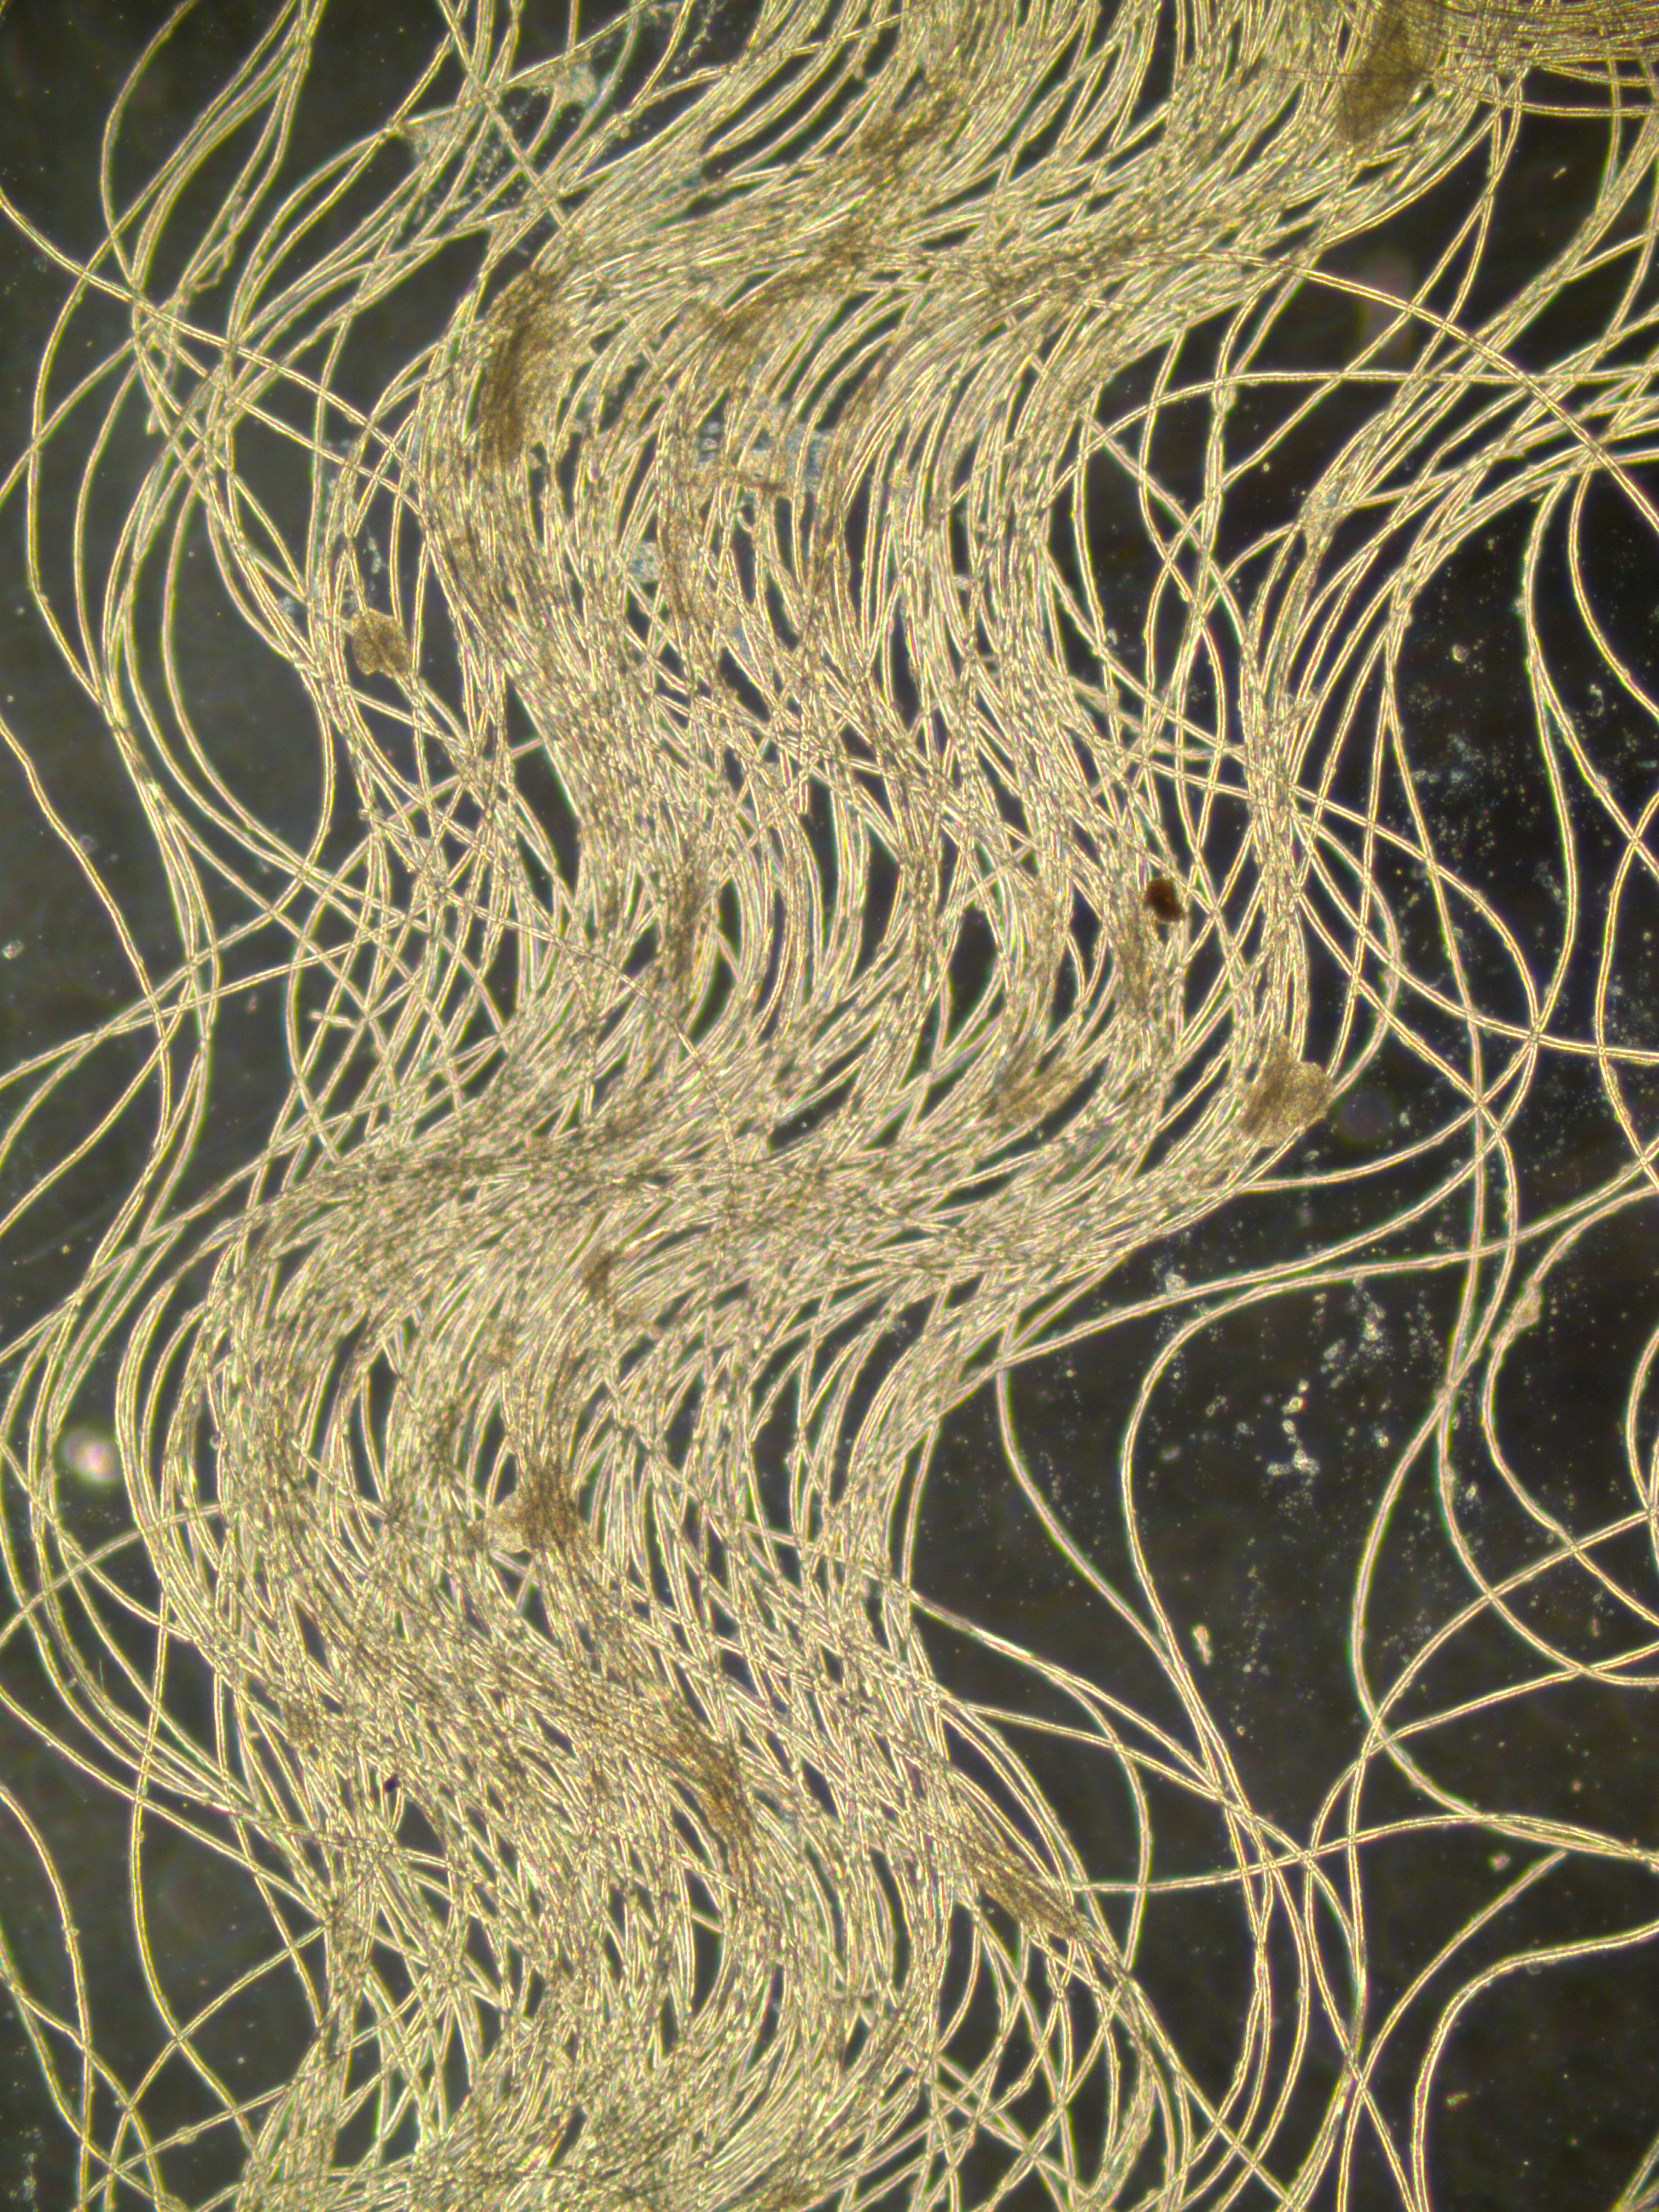
\includegraphics[scale=0.38]{figfibresstretchedrot.jpg}}\hfill
 \subfigure[Unfolded staple crimp type]{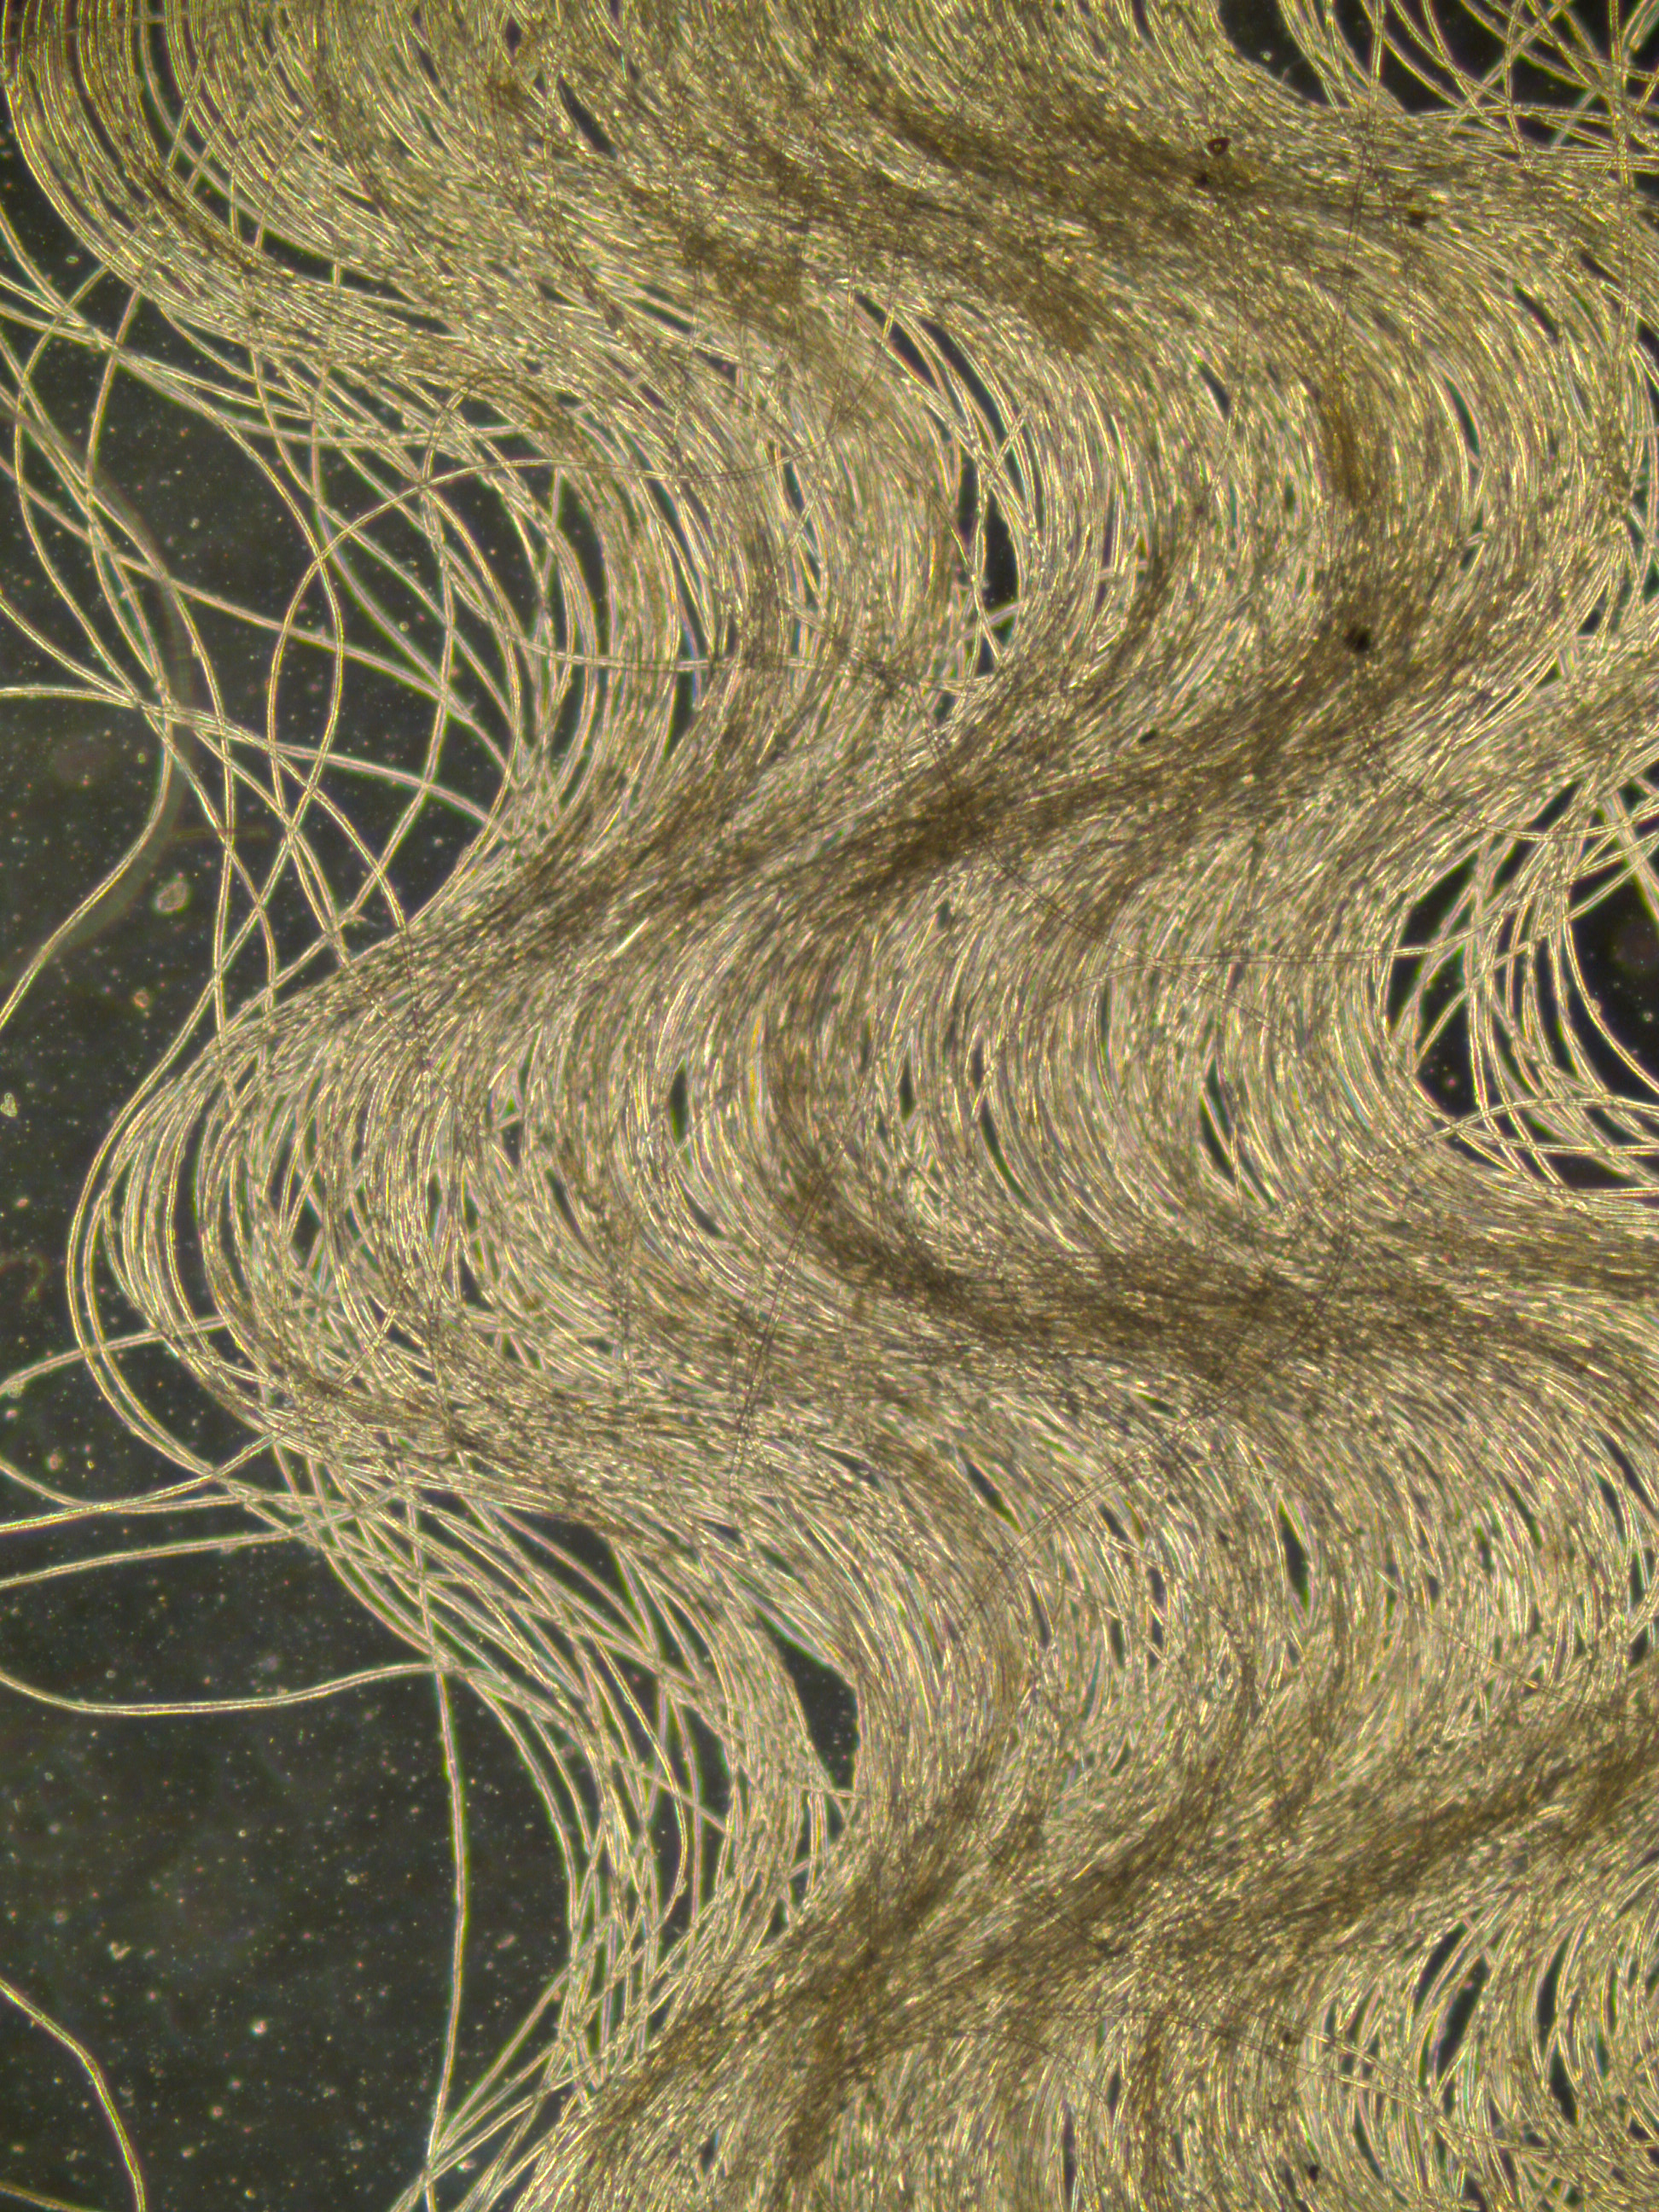
\includegraphics[scale=0.38]{figfibresunfoldedrot.jpg}}
\caption{Photomicrographs, taken with phase contrast microscope, showing multi
ple bundles of fibres for each of the three staple crimp types. Microscope magnification 25x. For printed magnification see Appendiox A.}
\label{fig:fibre3types}
\end{minipage}
\end{turn}
\end{figure}
%\end{document}
